\documentclass{article}\usepackage[]{graphicx}\usepackage[]{color}
%% maxwidth is the original width if it is less than linewidth
%% otherwise use linewidth (to make sure the graphics do not exceed the margin)
\makeatletter
\def\maxwidth{ %
  \ifdim\Gin@nat@width>\linewidth
    \linewidth
  \else
    \Gin@nat@width
  \fi
}
\makeatother

\definecolor{fgcolor}{rgb}{0.345, 0.345, 0.345}
\newcommand{\hlnum}[1]{\textcolor[rgb]{0.686,0.059,0.569}{#1}}%
\newcommand{\hlstr}[1]{\textcolor[rgb]{0.192,0.494,0.8}{#1}}%
\newcommand{\hlcom}[1]{\textcolor[rgb]{0.678,0.584,0.686}{\textit{#1}}}%
\newcommand{\hlopt}[1]{\textcolor[rgb]{0,0,0}{#1}}%
\newcommand{\hlstd}[1]{\textcolor[rgb]{0.345,0.345,0.345}{#1}}%
\newcommand{\hlkwa}[1]{\textcolor[rgb]{0.161,0.373,0.58}{\textbf{#1}}}%
\newcommand{\hlkwb}[1]{\textcolor[rgb]{0.69,0.353,0.396}{#1}}%
\newcommand{\hlkwc}[1]{\textcolor[rgb]{0.333,0.667,0.333}{#1}}%
\newcommand{\hlkwd}[1]{\textcolor[rgb]{0.737,0.353,0.396}{\textbf{#1}}}%
\let\hlipl\hlkwb

\usepackage{framed}
\makeatletter
\newenvironment{kframe}{%
 \def\at@end@of@kframe{}%
 \ifinner\ifhmode%
  \def\at@end@of@kframe{\end{minipage}}%
  \begin{minipage}{\columnwidth}%
 \fi\fi%
 \def\FrameCommand##1{\hskip\@totalleftmargin \hskip-\fboxsep
 \colorbox{shadecolor}{##1}\hskip-\fboxsep
     % There is no \\@totalrightmargin, so:
     \hskip-\linewidth \hskip-\@totalleftmargin \hskip\columnwidth}%
 \MakeFramed {\advance\hsize-\width
   \@totalleftmargin\z@ \linewidth\hsize
   \@setminipage}}%
 {\par\unskip\endMakeFramed%
 \at@end@of@kframe}
\makeatother

\definecolor{shadecolor}{rgb}{.97, .97, .97}
\definecolor{messagecolor}{rgb}{0, 0, 0}
\definecolor{warningcolor}{rgb}{1, 0, 1}
\definecolor{errorcolor}{rgb}{1, 0, 0}
\newenvironment{knitrout}{}{} % an empty environment to be redefined in TeX

\usepackage{alltt}
\usepackage{Sweave}
\usepackage{float}
\usepackage{graphicx}
\usepackage{tabularx}
\usepackage{siunitx}
\usepackage{geometry}
\usepackage{pdflscape}
\usepackage{mdframed}
\usepackage{natbib}
\bibliographystyle{..//refs/styles/besjournals.bst}
\usepackage[small]{caption}
\setlength{\captionmargin}{30pt}
\setlength{\abovecaptionskip}{0pt}
\setlength{\belowcaptionskip}{10pt}
\topmargin -1.5cm        
\oddsidemargin -0.04cm   
\evensidemargin -0.04cm
\textwidth 16.59cm
\textheight 21.94cm 
%\pagestyle{empty} %comment if want page numbers
\parskip 7.2pt
\renewcommand{\baselinestretch}{1.5}
\parindent 0pt
\usepackage{lineno}
\linenumbers

\newmdenv[
  topline=true,
  bottomline=true,
  skipabove=\topsep,
  skipbelow=\topsep
]{siderules}

%% R Script


\IfFileExists{upquote.sty}{\usepackage{upquote}}{}
\begin{document}
\title{Rethinking False Spring Risk}
\author{C. J. Chamberlain $^{1,2}$, B. I. Cook $^{3}$, I. Garcia de Cortazar Atauri $^{4}$, E. M. Wolkovich $^{1,2}$}
\date{\today}
\maketitle 
%\tableofcontents
 

\renewcommand{\thetable}{\arabic{table}}
\renewcommand{\thefigure}{\arabic{figure}}
\renewcommand{\labelitemi}{$-$}
\setkeys{Gin}{width=0.8\textwidth}

%%%%%%%%%%%%%%%%%%%%%%%%%%%%%%%%%%%%%%%%%%%%%%%
% General to do
% Move all figures and their captions to end of manuscript
% Work on transitions throughout. I made note of it many places.
% My comments are usually in [] and I made some edits throughout. You can use the app FileMerge (spotlight search for it) on most Macs to see the changes quickly. 
%%%%%%%%%%%%%%%%%%%%%%%%%%%%%%%%%%%%%%%%%%%%%%%


\section{Abstract}
Trees and shrubs growing in temperate environments are at risk of being exposed to late spring freezes, or false spring events, which can be damaging ecologically and economically. As climate change may alter the potential prevalence and severity of false spring events, our ability to accurately forecast such events has become more critical. Yet currently, false spring studies largely simplify the various ecological elements that could predict the level of plant damage from late spring freezing events. Here we review how to improve false spring equations for future projections. In particular we highlight how integrating species, life stage, and habitat differences could help accurately determine the level of damage sustained by a false spring event. %(The ultimate intent is to demonstrate how an integrated view of false spring that incorporates these factors would rapidly advance progress in this field.)
Integrating some of these complexities could help rapidly advance understanding and forecasting of false spring events in climate change and ecological studies.

\section{Introduction}

Plants growing in temperate environments time their growth each spring to follow rising temperatures and increasing light and soil resource availability. While tracking spring resource availability, temperate plants are at risk of late spring freezes, which can be detrimental to growth. Individuals that leaf out before the last freeze date are at risk of leaf loss, damaged wood tissue, and slowed or stalled canopy development \citep{Gu2008, Hufkens2012}. These damaging late spring freezing events are known as false springs, and are widely documented to result in highly adverse ecological and economic consequences \citep{Knudson2012, Ault2013}.

% EMW: Thanks for adding references to the temperature variation. Unfortunately I am not comfortable with these references, especially the Vasseur one (remind me and we can discuss briefly). I suggest you remove this one and add 1-2 from the climate literature. My understanding is temperature variation is not going to change that much in most regions, and I don't want to support a narrative that it will when it won't. An easy fix for now is deleting a couple sentences I am not sure we need (deleted below, see what you think). But in the longer run I suggest you Skype with Ben to discuss more and track down some balanced citations from the physical science literature.
Climate change is expected to cause an increase in damage from false spring events due to earlier spring onset and greater fluctuations in temperature in some regions \citep{Cannell1986, Inouye2008, Martin2010}. Already, multiple studies have documented false spring events in recent years \citep{Gu2008, Augspurger2009, Knudson2012, Augspurger2013} and some have linked these events to climate change \citep{Ault2013, Allstadt2015, Muffler2016, Xin2016}. This increasing interest in false spring events has led to a growing body of research investigating the effects on temperate forests and agricultural crops. But for this research to produce accurate predictions on future trends, researchers need methods that properly evaluate the effects of false spring events across the diverse species, habitats and climate regimes they are studying. 

Current metrics for estimating false springs events are generally simple: often requiring an estimate for the start of `spring' and whether temperatures occurred below a particular temperature threshold in the following week. Such estimates inherently assume consistency of responses across species, functional group, life stages, habitat type, and other climatic regimes, ignoring that such factors can greatly impact plants' false spring risk. As a result, such indices will most likely lead to inaccurate current estimates as well as poor future predictions, slowing our progress in understanding false spring events and how they may shift with climate change. 

In this paper we aim to highlight the complexity of factors driving a plant's false spring risk and provide a road map for improved metrics. First, we review the currently used definitions of false spring. Then, combining research from plant physiology, climatology and community ecology, we outline major gaps in current definitions. In particular we show how life stage \citep{Caffarra2011}, location within a forest or canopy \citep{Augspurger2013}, interspecific variation in avoidance and tolerance strategies (Flynn \& Wolkovich 2017?), freeze temperature thresholds, and regional effects \citep{Martin2010} unhinge simple metrics of false spring. We argue that a new approach that integrates these and other crucial factors would help accurately determine current false spring damage and improve predictions of spring freeze risk under a changing climate---while potentially providing novel insights to how plants respond to and are shaped by spring frost. % The ultimate intent is to demonstrate how an integrated view of false spring that incorporates these factors would rapidly advance progress in this field.  

\section{Defining False Spring: An example in one temperate plant community}
Temperate forest plants are most at risk to frost damage from episodic spring frosts \citep{Sakai1987}. Due to the stochastic nature of episodic spring frosts, plants must exhibit flexible spring phenologies in order to minimize freezing risk. Freezing temperatures following a warm spell could result in plant damage or even death \citep{Ludlum1968, Mock2007}. Intracellular ice formation from false spring events often results in severe leaf and stem damage. Ice formation can also occur indirectly (i.e. extracellularly), which results in freezing dehydration and mimics extreme drought conditions \citep{Pearce2001, Beck2004, Hofmann2015}. Both forms of ice formation can cause defoliation and, ultimately, crown dieback \citep{Gu2008}. Once buds exit the dormancy phase, they are less freeze tolerant and resistance to bud ice formation is greatly reduced \citep{Taschler2004, Lenz2013, Vitasse2014a}. An effective and consistent definition of false spring that more accurately determines the amount and type of ice formation is essential to properly evaluate the level of damage that could occur.

% EMW: Tiny edits below...
There are several definitions currently used to define a false spring. A common definition describes a false spring as having two phases: rapid vegetative growth prior to a freeze and a post freeze setback \citep{Gu2008}. Other definitions instill more precise temporal parameters, specific to certain regions \citep[e.g., in][false spring for the Midwestern United States is defined as a warmer than average March, a freezing April, and enough growing degree days between budburst and the last freeze date]{Augspurger2013}. A widely used definition integrates a mathematical equation to quantify a false spring event. This equation, known as a False Spring Index (FSI), signifies the likelihood of a damage to occur from a late spring freeze. Currently, FSI is evaluated by the day of budburst and the day of last spring freeze through a simple equation as seen below \citep{Marino2011}. 
\begin{equation} \label{eq:1}
FSI = \text{Day of Year} (Last Spring Freeze) - \text{Day of Year} (Budburst)
\end{equation}
A damaging FSI is currently defined to be 7 or more days between budburst and the last freeze date (Equation \ref{eq:1}) \citep{Peterson2014}. The 7 day parameter exposes less resistant foliate phenophases to a false spring, thus putting the plant at a higher risk of damage. 

To demonstrate how the FSI definition works, we applied it to data from the Harvard Forest Long-term Ecological Research program in Massachusetts. We used three separate methodologies to calculate spring onset: long-term ground observational data \citep{Okeefe2014}, PhenoCam data from Harvard Forest \citep{Richardson2015}, and USA National Phenology Network (USA-NPN) Extended Spring Index (SI-x) data \citep{USA-NPN2016}. These spring onset values were then inputted into the FSI equation (Equation \ref{eq:1}) to calculate FSI from 2008 to 2014 (Figure \ref{fig:fsifig}). 

% EMW: Tiny edits below...
Each methodology renders different FSI values, suggesting different false spring damage for the same site and same year. For most years, the observational FSI and PhenoCam FSI are about 10-15 days lower than the SI-x data. This is especially important for 2008, when the SI-x data indicates a false spring year, whereas the other two datasets do not. In 2012, the observational data and PhenoCam data diverge and the PhenoCam FSI is over 30 days less than the SI-x value.

The reason for these discrepancies is that each method evaluates spring onset for different species or functional groups within a forest community. Spring phenology in temperate forests typically progresses by functional group: understory species and young trees tend to initiate budburst first, whereas larger canopy species may start later in the season \citep{Richardson2009, Xin2016}. The different FSI values determined in Figure \ref{fig:fsifig} exemplify the differences in functional group spring onset dates and illustrate variations in forest demography and phenology, which is most apparent in 2012. In 2012, a false spring event was reported through many regions of the US due to warm temperatures occurring in March \citep{Ault2015}. These high temperatures would most likely be too early for larger canopy species to initiate budburst but they would affect smaller understory species as is seen in Figure 1. 

% EMW: Tiny edits below...
Yet, in contrast to our three metrics of spring onset for one site, most FSI work currently ignores variation across functional groups --- instead using one metric of spring onset and assuming it applies to the whole community of plants. The risk of a false spring varies across habitats and with species composition since spring onset is not consistent across functional groups. Therefore, one spring onset date cannot be used as an effective proxy for all species. False spring studies should first assess the forest demographics and functional groups relevant to the study question in order to effectively estimate the date of spring onset. However, as we outline below, considering different functional groups is unlikely to be enough for robust predictions. It is also crucial to integrate species differences within functional groups and consider the various interspecific avoidance and tolerance strategies against false springs. %EMW cut after re-order: ... equation is built half on spring onset date, it is critical to choose the most appropriate methodology that targets the species of interest within the study. 

\section {Plant Physiology and Diversity versus the Current False Spring Definition}
% EMW: Tiny edits below...
Plants have evolved to minimize false spring damage through two strategies: avoidance and tolerance. Effective avoidance strategies require well-timed spring phenologies. Temperate deciduous tree species optimize growth and minimize spring freeze damage by using three cues to initiate budburst: low winter temperatures, warm spring temperatures, and increasing photoperiods \citep{Chuine2010}. The evolution of these three cues and their interactions has permitted temperate plant species to occupy more northern ecological niches and decrease the risk of false spring damage, which is crucial for avoidance strategies \citep{Samish1954}. One avoidance strategy, for example, is the interaction between over-winter chilling and spring forcing temperatures. Warm temperatures earlier in the year (i.e. in February) will not result in early budburst due to insufficient chilling \citep{Basler2012}. Likewise, photoperiod sensitivity is a common false spring avoidance strategy: species that respond strongly to photoperiod cues in addition to warm spring temperatures will likely delay budburst and evade false spring events as spring continues to advance earlier in the year \citep{Basler2014}. 

Some temperate forest species have evolved to be more tolerant of spring freezing temperatures, rather than try to avoid frosts via more flexible phenologies. Temperate forest plants utilize various morphological strategies to be more frost tolerant: some have toothed or lobed leaves to increase `packability' in winter buds, which permits more rapid leafout and minimizes exposure time of less resistant tissues \citep{Edwards2017}. Other species have young leaves with more trichomes to act as a buffer against spring frosts \citep{Agrawal2004}, and many are able to respond to abiotic cues such as consistently dry winters. Species living in habitats with drier winters develop shoots and buds with decreased water content, which makes the buds more tolerant to drought and also to false spring events \citep{Beck2007, Morin2007, Nielsen2009, Poirier2010, Kathke2011, Hofmann2015}. More studies are needed to investigate the interplay between false spring events, leaf morphology, and precipitation and how these relationships affect false spring tolerance. Given the diverse array of spring freezing defense mechanisms, predicting damage by false spring events requires a greater understanding of avoidance and tolerance strategies across species, especially with a changing climate.

\section {Defining Vegetative Risk: Complexities due to Species' Strategies and Climate}
% EMW: Tiny edits below...
Phenology and frost tolerance are intertwined---with important variation occurring both across and within different phenological events. Different phenological phases respond differently to false spring events. Flowering and fruiting phenophases are generally more sensitive than vegetative phases \citep{Augspurger2009, Lenz2013}. %(Damage to flowers and fruits can hinder reproductive growth for that entire season. However,)
False spring events that occur during the vegetative growth phenophases impose the greatest freezing threat to deciduous tree and shrub species because plants will suffer greater long-term effects from the loss of photosynthetic tissue, which could impact multiple years of growth, reproduction, and canopy development \citep{Sakai1987, Vitasse2014}. Within certain phenological phases (i.e. before full leafout of the entire plant) plants are more likely to sustain damage from a false spring than individuals past the leafout phenophase. Spring phenology is thus a crucial measure for how much damage a plant will sustain from a freezing event.

% EMW: Tiny edits below... please check my 'e.g.' edit to make sure it is correct
Freezing tolerance steadily decreases after budburst begins until the leaf is fully unfolded \citep{Lenz2016} (Figure \ref{fig:risk}). Therefore, the rate of budburst and the length of time between budburst and leafout is essential for predicting level of damage from a false spring event. We will refer to the timing of these collective phenophases (i.e. budburst to leafout) as the duration of vegetative risk. The duration of vegetative risk is usually extended if a freezing event occurs during the phenophases between budburst and full leafout \citep{Augspurger2009}. One hypothesis suggests that species with short durations of vegetative risk often sustain higher levels of damage because more sensitive tissues will be exposed to frost. But if the duration of vegetative risk is longer, then the less vulnerable phenophases (e.g., full leafout) will be exposed to the frost for longer thus potentially minimizing the risk of damage \citep{Augspurger2009}. 

% EMW: Good improvements here but feels like it still needs a tweak or two, see comments embedded below.
Climate change further complicates understanding species vulnerabilities to spring frost between budburst and leafout. Most species are expected to begin leafout earlier in the season with warming spring temperatures but some species may have the opposite response due to less winter chilling or decreased photoperiod cues \citep{Cleland2006, Yu2010, Xin2016}. 
% EMW: Above seems great but there is a connection missing to the below -- it seems to touch on mostly stuff you have already mentioned: shorter DVR, other cues that let species avoid etc.. I suspect in your head these all link to climate change but there is no clear link for the reader. You may want to cut some sentences and use the rest to make clear what your point is -- are you identifying which types of species are at the biggest risk in the future with climate change and/or are you trying to layout the complexities that make prediction hard? I think you are trying to do the latter and that you have set up 3 key effects: (1) DVR, (2) Regional effects and (3) species-level effects. You might need to spell out to the reader that all these things matter to predicting impacts with climate change ... and then you should keep them in the order they will next be presented (I think).
Individuals that initiate budburst earlier in the spring may attempt to limit freezing risk by decreasing the duration of vegetative risk in order to minimize the exposure of less frost tolerant phenophases. Alternatively, studies indicate that species growing at more northern latitudes tend to respond more to photoperiod than species growing further south and, subsequently, these species may have a longer durations of vegetative risk \citep {Partanen2004, Viheraaarnio2006, Caffarra2011}. Furthermore, larger canopy species exhibit greater photoperiod sensitivities than shade tolerant or understory species \citep{Basler2012} and they also, generally, require more chilling in the winter and greater forcing temperatures in the spring to initiate budburst \citep{Laube2013}.  
% EMW: Need better transition into this.
We assessed climate data across Europe, long-term observational data, and experimental data to gain a better understanding of the the interaction between duration of vegetative risk and false spring events.  '

\subsection {Predictable Regional Differences in Climate, Species Responses and False Spring Risk}
% EMW: Add citation  to variability sentences? Lots of chilling studies on coastal versus inland sites note this so good to cite one. You might even want to mention this as a known finding relating to false spring here and use it to transition to next paragraph.
Numerous studies have investigated the the relationship between budburst and photoperiod by using latitudinal gradients \citep{Partanen2004, Viheraaarnio2006, Caffarra2011, Zohner2016, Gauzere2017}, however few have integrated longitudinal variation or regional effects. Yet climate and thus false spring risk varies across regions. For example, consider five archetypal regions within a temperate climate. Some regions may experience harsher winters and greater temperature variability throughout the year than others, and these more variable regions often have a much higher risk of false spring (i.e. Maine) than others (i.e. Lyon). %(Figure \ref{fig:regional}). 
Understanding and integrating such spatiotemporal effects and regional differences when investigating false spring risk and duration of vegetative risk would help improve predictions as climate change progresses.
% [This can go in caption and should reference a supplement with the data sources and any relevant methods.] By determining the average time of budburst to leafout dates for the dominant species in five archetypal climate regions, we were able to estimate the current spatial variation of false spring risk (Figure \ref{fig:regional}). We assessed the number of freeze days (-2.2$^{\circ}$C) \citep{Schwartz1993} that occurred on average over the past 50 years within the average durations of vegetative risk for each region. 

% EMW: Edits below...
Predictions will want to consider carefully how chilling and forcing, which are key drivers of budburst and leafout, vary significantly across a longitudinal gradient. Climatic variation across regions results in varying durations of vegetative risk due to different chilling and forcing temperatures. It is therefore important to recognize climate regime extremes (e.g. seasonal trends, annual minima and annual maxima) in future studies in order to better understand the interplay between duration of vegetative risk and climatic variation. Different habitats exhibit variations in the amplitude of temperature variation, which could provide insight in the relationship between spring plant phenology and false spring risk. The climatic implications of advancing forcing temperatures could potentially lead to earlier dates of budburst and enhance the risk of frost. These shifts in climatic regimes could vary in intensity across regions (i.e. habitats currently at risk of false spring damage could become low risk regions over time). 

There are also discrepancies in defining a false spring event, especially with understanding damaging freezing temperatures. Some regions and species may tolerate lower temperature thresholds than others (Figure \ref{fig:temp}). Not only is there debate on what a damaging temperature threshold is, but it is still not well understood how the damage sustained relates to the duration of the frost \citep{Sakai1987, Augspurger2009, Vitasse2014, Vitra2017}. It is crucial to gain an understanding on which climatic parameters result in false spring events and how these parameters may vary across regions. It is anticipated that most regions will have earlier spring onsets, however, last freeze dates will not advance at the same rate \citep{Inouye2008,Martin2010,Labe2016}, rendering some regions and species to be more susceptible to false spring events in the future. 

\subsection{Changes in Phenological Cues and the Duration of Vegetative Risk}
% EMW: Tiny edits below...
The risk of false spring may shift as climate change progresses and greater forcing temperatures occur earlier in the year. Studies suggest that spring forcing temperatures directly affect the duration of vegetative risk: years with lower forcing temperatures and fewer growing degree days will have longer durations of vegetative risk \citep{Donnelly2017}. With spring advancing, it is anticipated that there will be greater fluctuations in spring forcing temperatures \citep{Martin2010}. These fluctuations in spring temperature are expected to oscillate above and below the development threshold within a spring season. With less consistent forcing temperatures, we would expect to see longer durations of vegetative risk in a changing climate. Therefore, it is hypothesized that the species able to track the shifts in spring advancement due to climate change will be more susceptible to false spring damage \citep{Scheifinger2003}. We investigated this interaction using observational data from Harvard Forest \citep{Okeefe2014} and compared two years of data: one year that had an unusually early spring onset (2010) and another year that an unusually late spring onset (2014).

By comparing the durations of vegetative risk to the growing degree days for each year, we found that the number of growing degree days were highly comparable for both years (Figure \ref{fig:forest}). Observational data failed to demonstrate the expected result. However, phenological data in an experimental context suggests differently. %% Not sure how to really wrap this up... thinking of investigating a new relationship -- do false spring years cause individuals to leaf out later the next year? Maybe look at GDD trends from year to year using John's data and weather data.

% \subsection{Interaction of Phenological Cues and the Duration of Vegetative Risk}
% EMW: Check out edits below...
Each species responds differently to climate change, therefore, the duration of vegetative risk depends on the interaction between cues and species. [Species dominated by forcing cues may shift earlier and earlier with climate change but most species also have photoperiod and chilling cues, which complicate predictions.] For example, as climate change progresses, higher spring forcing temperatures may be required for species experiencing insufficient winter chilling (due to warmer winter temperatures), especially at lower latitudes \citep{McCreary1990, Morin2009, Fu2012, Polgar2014, Chuine2010}. Anthropogenic climate change will cause changes in winter and spring temperatures, resulting in greater differences in spring phenology cue requirements across species and regions. This interaction of cues---and how climate change will affect that interaction---is crucial for recognizing which species will likely become more at risk of false spring events in the future.
% EMW cut: Spring forcing temperatures and day length requirements for budburst to occur vary among species and across habitats [this is basically a repeat of your first sentence here]. Since species distributions are largely driven by phenology \citep{Chuine2001}, species less reliant on photoperiod cues are likely to outcompete species that are reliant on photoperiod cues as spring forcing temperatures continue to initiate earlier \citep{Vitasse2011, Gauzere2017}. [This next sentence did not feel super relevant for this paper. I totally see your point but it is a whole other topic -- community shifts -- to throw in in just one sentence.]

We assessed data from a growth chamber experiment in order to investigate the interaction of cues across species and predict potential shifts in duration of vegetative risk with climate change. We compared 9 temperate forest species between two treatments: high chilling hours, long photoperiod and high forcing temperatures (WL1) against no additional chilling, short photoperiod and low forcing temperatures (CS0) (Flynn and Wolkovich, 2017?). According to the results, individuals that initiate budburst earlier in the season (i.e. {\textit {Betula papyrifera}} (Marsh.) and {\textit{Ilex mucronata}} (L.)) tend to initiate budburst early regardless of treatment, but the treatment does affect the duration of vegetative risk significantly (Figure \ref{fig:dan}). As the season progresses, treatment does not affect the duration of vegetative risk as much but the day of budburst tends to be later in the season with the weaker treatment effects (i.e. CS0). Anova results indicate forcing temperatures and photoperiod length determine the duration of vegetative risk more than chilling requirements. This could suggest that chilling influences budburst and leafout similarly, while photoperiod and forcing temperatures have varying effects on the two phenophases. With a changing climate, forcing temperatures will increase and initiate earlier in the season while photoperiod cues will remain stagnant or decrease. This cue interaction could potentially elongate the duration of vegetative risk and expose at risk plants to more intense false spring events or even multiple events in one year. Further studies are essential to investigate the interplay between chilling, forcing, and photoperiod cues on the duration of vegetative risk, especially for species occupying ecological niches more susceptible to false spring events. 

\section{Conclusion}
% EMW: May want to double-check you hit all your major points here, and not just a (random?) subset of them....
The risk of false spring damage varies across years and regions and the timing between last freeze date and date of spring onset may become less consistent. With warm temperatures advancing in the spring but last spring freeze dates staying the same, there could potentially be more damaging events in the future, especially in high risk regions \citep{Gu2008, Inouye2008}. By utilizing only two simple metrics (last freeze date and spring onset date), researchers fail to assess the myriad of factors essential in determining false spring risk and damage. Future studies are necessary to gain an understanding with relationships between species, functional group, phenophase, and region and the differences in false spring damage. It is also essential that a temperature threshold is established for all functional types and phenophases across regions in order to effectively predict false spring risk in the future. An integrated approach to assessing past and future spring freeze damage must be realized as global climate change progresses in order to mitigate the adverse ecological and economic effects of false springs.
% EMW: Cut below, feels like a lot of new info to have in a conclusion section. 
% This shift in timing could result in more events where understory species leaf out prior to the last freeze and escape frost damage but canopy species may be at higher risk, thus potentially resulting in crown dieback for the larger tree species and subsequently enhanced sun exposure and damage to understory species. For these reasons, a greater understanding of false spring damage as climate change progresses is necessary.



\bibliography{..//refs/SpringFreeze.bib}

\begin{figure}[H]

{\centering 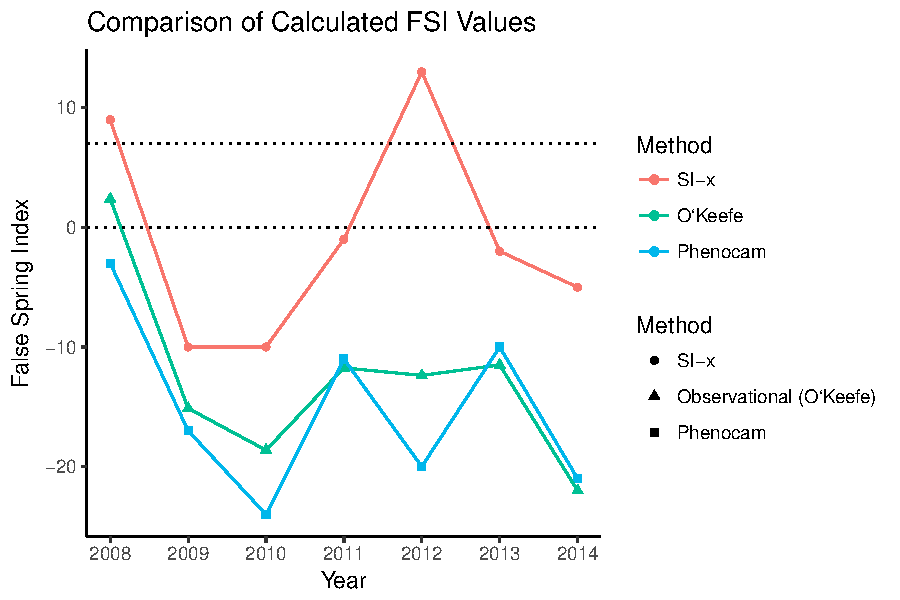
\includegraphics[width=\maxwidth]{figure/fsifig-1} 

}

\caption[A scatterplot indicating FSI values from 2008 to 2014 for each methdology used in this study]{A scatterplot indicating FSI values from 2008 to 2014 for each methdology used in this study. USA-NPN FSI values are green (USA-NPN, 2016), observed FSI values are blue (O'Keefe, 2014), and PhenoCam FSI values are red (Richardson, 2015).}\label{fig:fsifig}
\end{figure}




\begin{knitrout}
\definecolor{shadecolor}{rgb}{0.969, 0.969, 0.969}\color{fgcolor}\begin{kframe}
\begin{verbatim}
## lmer(formula = risk ~ chilling + warm + photo + (chilling + warm + 
##     photo | species), data = dxx)
##             coef.est coef.se
## (Intercept) 53.35     6.15  
## chilling    -0.10     0.36  
## warm        -1.54     0.19  
## photo       -1.19     0.15  
## 
## Error terms:
##  Groups   Name        Std.Dev. Corr              
##  species  (Intercept) 17.27                      
##           chilling     0.61    -0.73             
##           warm         0.50    -1.00  0.78       
##           photo        0.29    -0.98  0.84  0.99 
##  Residual              7.44                      
## ---
## number of obs: 996, groups: species, 9
## AIC = 6896.2, DIC = 6861.6
## deviance = 6863.9
\end{verbatim}
\end{kframe}
\end{knitrout}

\begin{figure} [H] 
\begin{center}
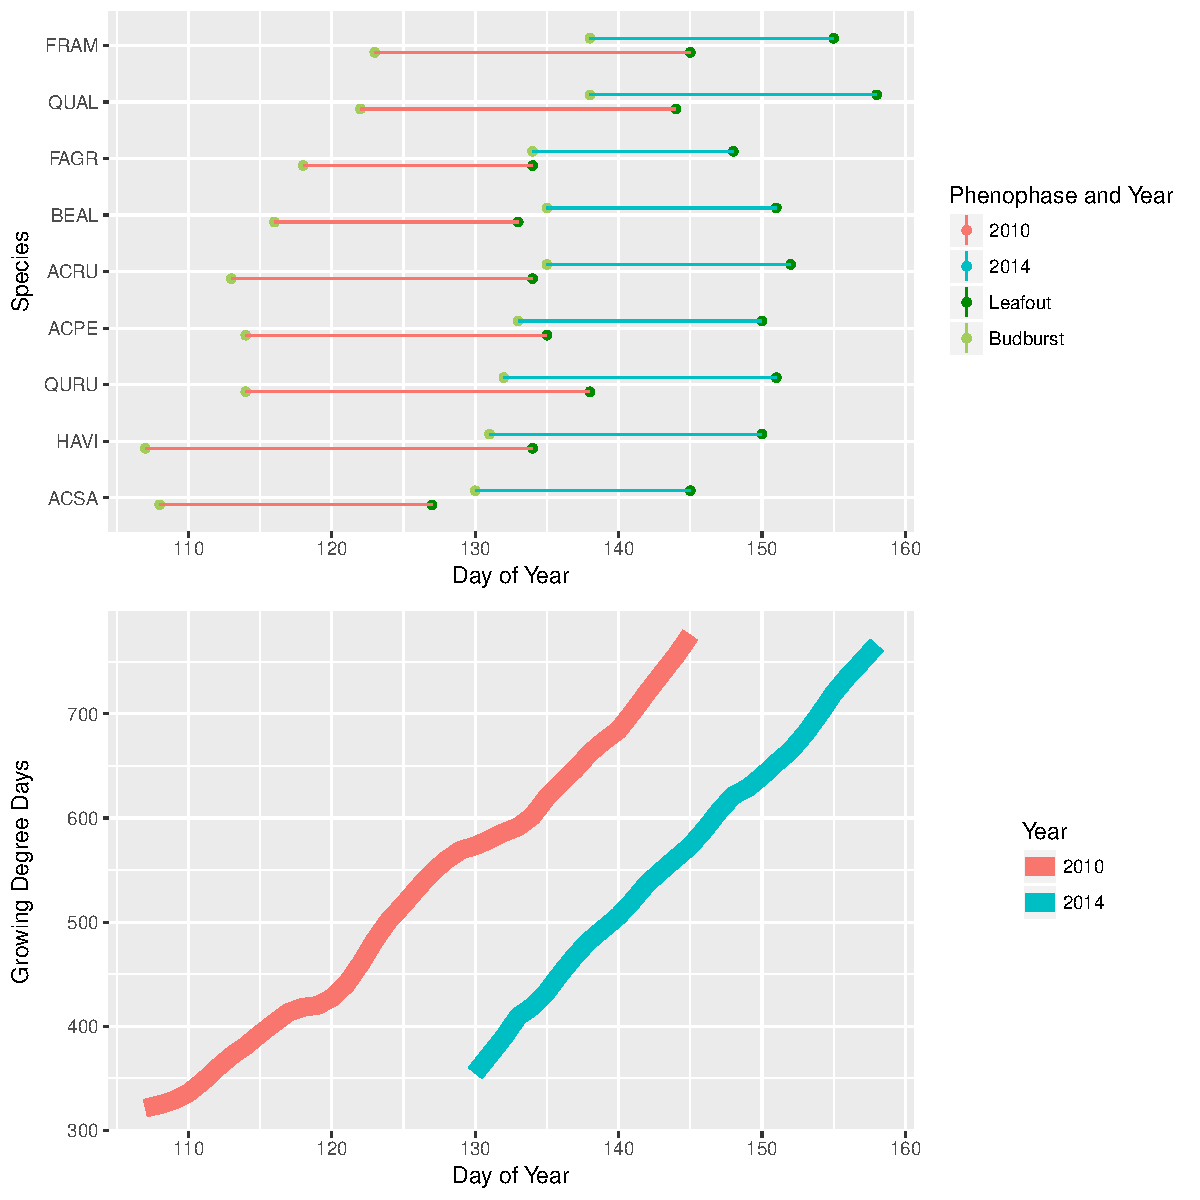
\includegraphics{..//figure/HF_gddTime.pdf}
\caption{A comparison of two years of observational data investigating the effects of growing degree days on the duration of vegetative risk. The average duration of vegetative risk for 2010 was 21 +/- 3.39 days versus 17.1 +/- 1.96 days in 2014.}\label{fig:forest}
\end{center}
\end{figure}

\begin{kframe}


{\ttfamily\noindent\bfseries\color{errorcolor}{\#\# Error in file(file, "{}rt"{}): cannot open the connection}}\end{kframe}\begin{figure}[H]

{\centering 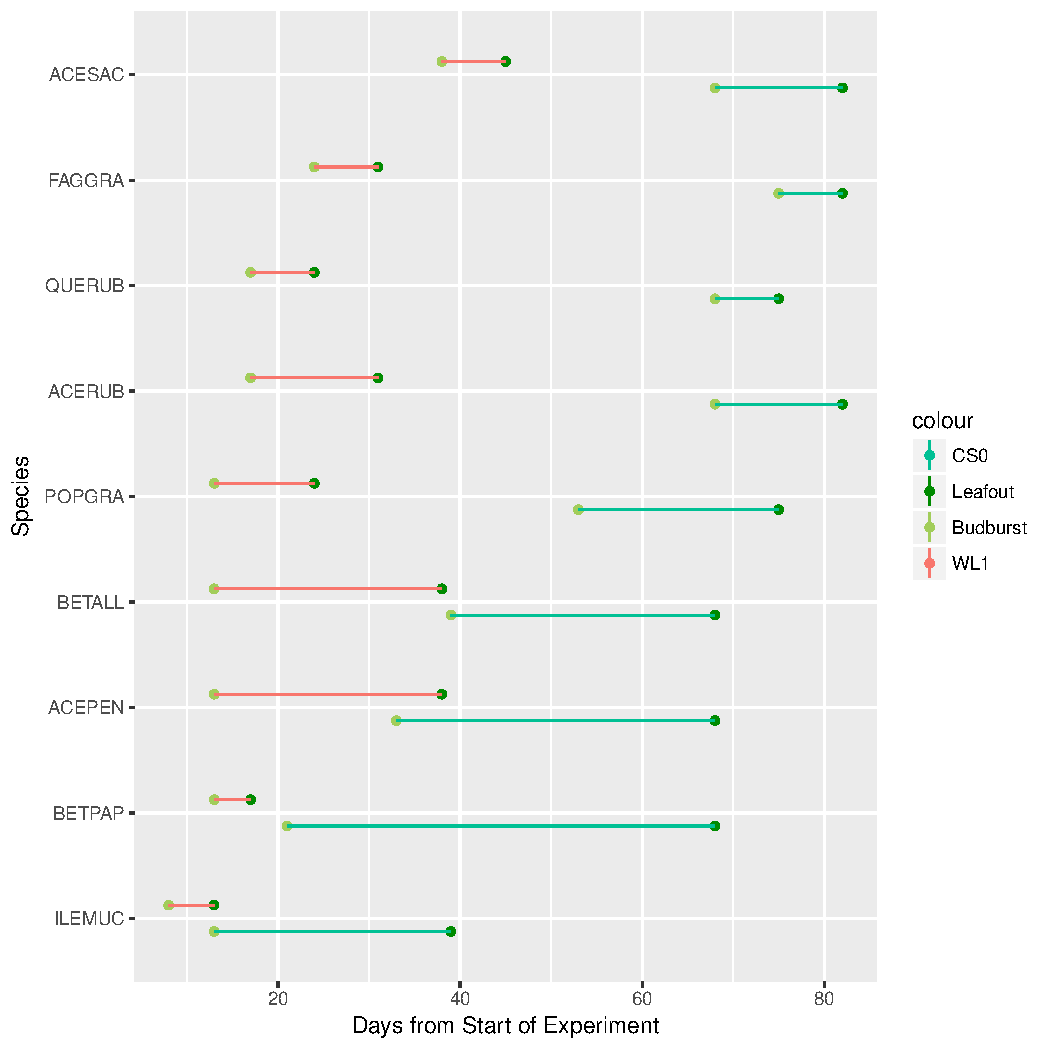
\includegraphics[width=\maxwidth]{figure/dan-1} 

}

\caption[This figure is comparing difference in duration of vegetative risk across two treatments for each species collected for the experiment]{This figure is comparing difference in duration of vegetative risk across two treatments for each species collected for the experiment. Data was collected from a growth chamber experiment where one treatment had no additional overwinter chilling, low spring forcing temperatures, and shorter spring daylengths and the other had additional overwinter chilling, high spring forcing temperatures, and longer spring daylenghts. The standard error is represented by the bars around each point.}\label{fig:dan}
\end{figure}



\begin{figure}[H]

{\centering 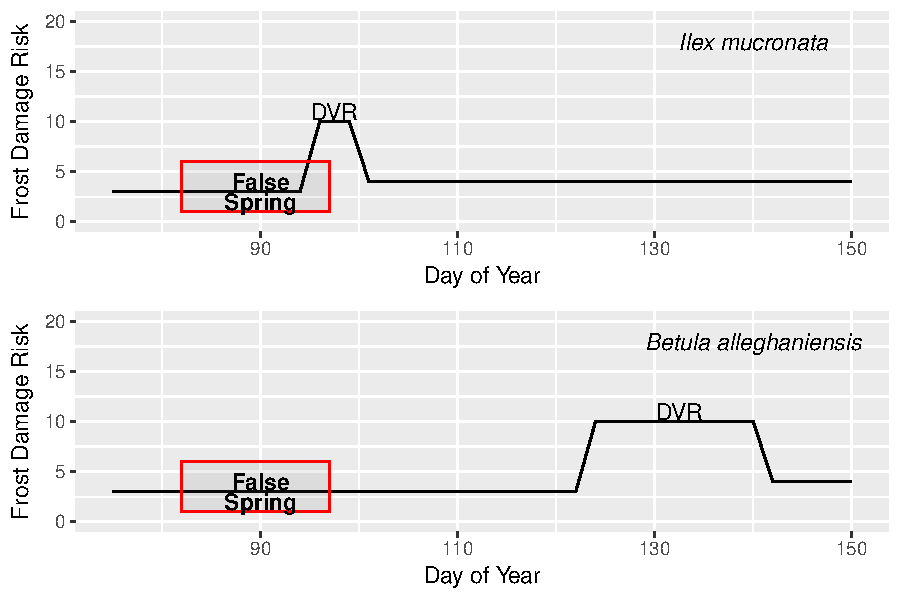
\includegraphics[width=\maxwidth]{figure/risk-1} 

}

\caption{A figure showing the differences in spring phenology and false spring risk across two species: \textit{Ilex mucronata} and \textit{Betula alleghaniensis}. We mapped a possible false spring event based on historic weather data and compared it to the observational data collected at Harvard Forest (O'Keefe, 2014). In this scenario, the \textit{Ilex mucronata} would be exposed to a false spring event, whereas the \textit{Betula alleghaniensis} would avoid it entirely. DVR stands for Duration of Vegetative Risk.}\label{fig:risk}
\end{figure}



\begin{figure}[H]

{\centering 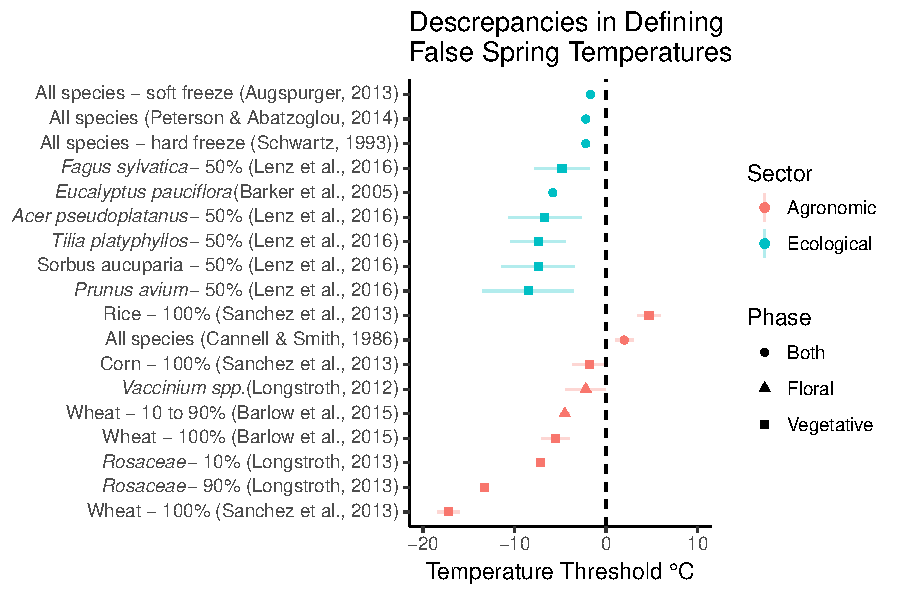
\includegraphics[width=\maxwidth]{figure/temp-1} 

}

\caption[A comparison of damaging spring freezing temperature thresholds across ecological and agronomic studies]{A comparison of damaging spring freezing temperature thresholds across ecological and agronomic studies. Each study is listed on the y axis along with the taxonimic group of focus. Next to the species name is the freezing definition used within that study (e.g. 100\% is 100 lethality). Each point is the best estimate recorded for the temperature threshold with standard deviation if indicated in the study. The shape of the point represents the phenophases of interest and the colors indicate the type of study (i.e. agronomic or ecological).}\label{fig:temp}
\end{figure}


\end{document}
